\documentclass{report}
\usepackage[utf8]{inputenc}
\usepackage{graphicx}
\usepackage{float}
\usepackage[a4paper]{geometry}
\usepackage{listings}
\usepackage{color}
\usepackage{subfig}
\usepackage{acro}
\usepackage{wrapfig}
\usepackage{multicol}
\usepackage{multirow}
\usepackage{bm}
\geometry{verbose,tmargin=3cm,bmargin=4cm,lmargin=2.5cm,rmargin=3cm}
\setcounter{secnumdepth}{3}
\setcounter{tocdepth}{3}
\usepackage[autostyle=true]{csquotes}
\usepackage{textcomp}
\usepackage[unicode=true,
 bookmarks=true,bookmarksnumbered=false,bookmarksopen=false,
 breaklinks=false,pdfborder={0 0 1},backref=false,colorlinks=false]
 {hyperref}
\usepackage{url}
\usepackage{hyperref}
\usepackage{graphicx}
\usepackage{amsmath}
\usepackage{mathtools}
\usepackage{tabularx,colortbl}
\usepackage[table]{xcolor}
\usepackage[labelfont=bf]{caption}
\usepackage{icomma} %Fjerner spacing etter komma
\usepackage[final]{pdfpages} %for å inkludere pdf-er. 
%bruk dette for å inkludere: \includepdf[pages=-]{file.pdf}

% Disse kommandoene kan gjøre det enklere for LaTeX å plassere figurer og tabeller der du ønsker.
\setcounter{totalnumber}{5}
\renewcommand{\textfraction}{0.05}
\renewcommand{\topfraction}{0.95}
\renewcommand{\bottomfraction}{0.95}
\renewcommand{\floatpagefraction}{0.35}

%Colors
\definecolor{brandeisblue}{rgb}{0.0, 0.44, 1.0}
\definecolor{blizzardblue}{rgb}{0.67, 0.9, 0.93}
\definecolor{beaublue}{rgb}{0.74, 0.83, 0.9}
\definecolor{orange}{RGB}{255,127,0}
\definecolor{denim}{rgb}{0.18, 0.48, 0.74}
\definecolor{deepskyblue}{rgb}{0.0, 0.75, 1.0}
\definecolor{lightcornflowerblue}{rgb}{0.6, 0.81, 0.93}
\definecolor{lblue}{rgb}{0.5, 0.71, 0.93}

\makeatletter
\makeatother



% probably a good idea for the nomenclature entries:
\acsetup{first-style=short}

% class `abbrev': abbreviations:
\DeclareAcronym{nzeb}{
  short = nZEB ,
  long  = net Zero Energy Building ,
  class = abbrev
}

\DeclareAcronym{npv}{
  short = NPV ,
  long  = Net present value ,
  class = abbrev
}

\DeclareAcronym{co2}{
  short = CO$_2$ ,
  long  = carbon dioxide ,
  class = abbrev
}

\DeclareAcronym{pv}{
  short = PV ,
  long  = Photovoltaics ,
  class = abbrev
}

\DeclareAcronym{hp}{
    short = HP ,
    long = Heat Pump ,
    class = abbrev
}

\DeclareAcronym{ASHP}{
    short = ASHP ,
    long = Air Source Heat Pump ,
    class = abbrev
}

\DeclareAcronym{COP}{
    short = COP ,
    long = Coefficient of Performance ,
    class = abbrev
}

\DeclareAcronym{Mtoe}{
    short = Mtoe ,
    long = Million Tonnes of Oil Equivalent ,
    class = abbrev
}

\DeclareAcronym{TRNSYS}{
    short = TRNSYS ,
    long = Transient Systems Simulation Program ,
    class = abbrev
}

\DeclareAcronym{AHU}{
    short = AHU ,
    long = Air Handling Unit ,
    class = abbrev
}

\DeclareAcronym{CAV}{
    short = CAV ,
    long = Constant air volume ,
    class = abbrev
}

\DeclareAcronym{VAV}{
    short = VAV ,
    long = Variable air volume ,
    class = abbrev
}

\DeclareAcronym{DCV}{
    short = DCV ,
    long = Demand controlled ventilation ,
    class = abbrev
}

\DeclareAcronym{pmv}{
    short = PMV ,
    long = Predicted mean vote ,
    class = abbrev
}

\DeclareAcronym{PPD}{
    short = PPD ,
    long = Predicted percentage of dissatisfied ,
    class = abbrev
}

% class `nomencl': nomenclature
\DeclareAcronym{investment}{
  short = \ensuremath{I} ,
  long  = Investment costs [NOK],
  sort  = I ,
  class = nomencl
}
\DeclareAcronym{lifetime}{
  short = \ensuremath{n} ,
  long  = Economic lifetime [years],
  sort  = n ,
  class = nomencl
}
\DeclareAcronym{balance}{
  short = \ensuremath{B} ,
  long  = Yearly balance [NOK],
  sort  = B ,
  class = nomencl
}

\DeclareAcronym{realrate}{
  short = \ensuremath{r} ,
  long  = Real rate of return [\%],
  sort  = r ,
  class = nomencl
}
\DeclareAcronym{Q}{
  short = \ensuremath{Q} ,
  long  = Heat [kW],
  sort  = Q ,
  class = nomencl
}

\DeclareAcronym{W}{
  short = \ensuremath{W} ,
  long  = Work [kW],
  sort  = W ,
  class = nomencl
}

\DeclareAcronym{To}{
  short = \ensuremath{t_o} ,
  long  = Operative temperature [$^o$C],
  sort  = t$_o$ ,
  class = nomencl
}

\begin{document}

%Forside
\pagestyle{empty} %No headings for the first pages.
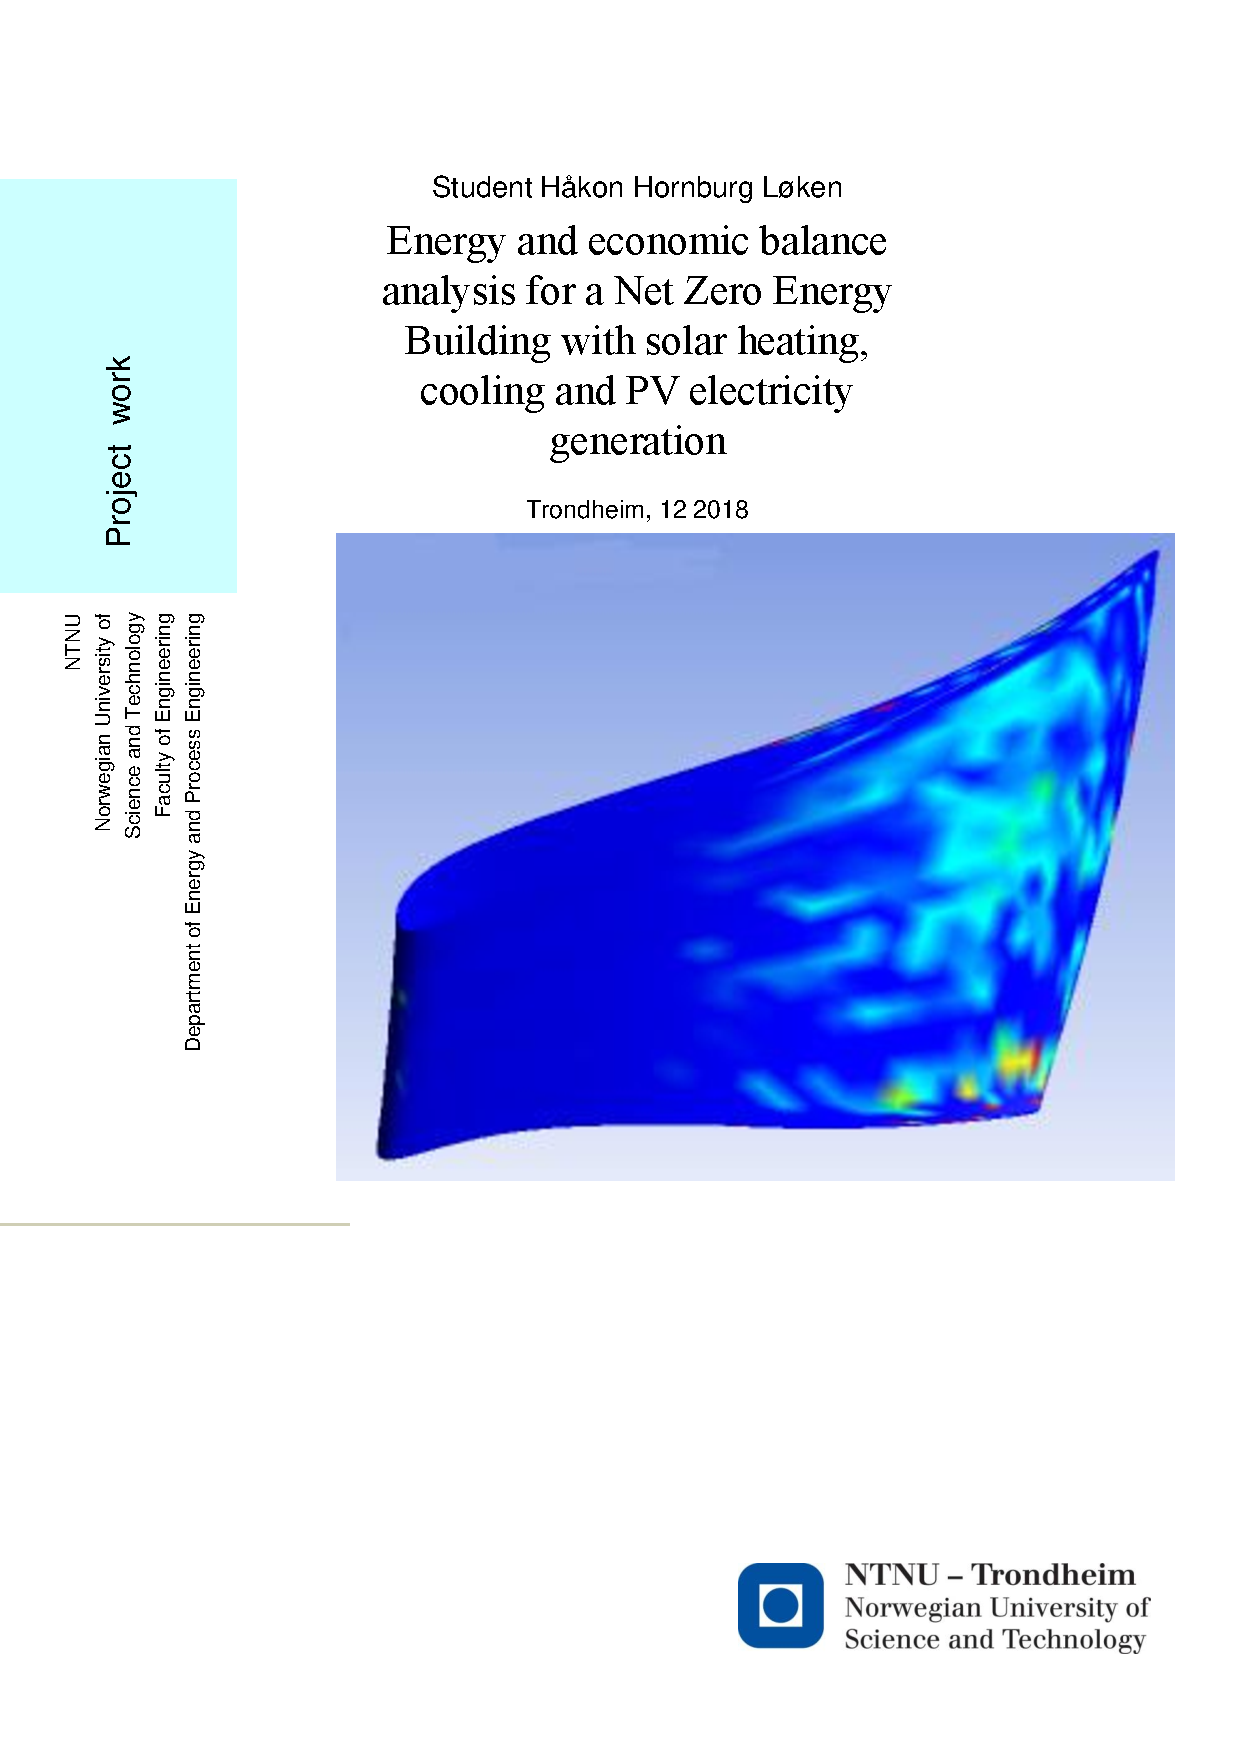
\includepdf[pages={1}, pagecommand={}]{vedlegg/Cover3.pdf}
\clearpage
\thispagestyle{empty}
\newpage

%Tom side
\pagestyle{empty} %No headings for the first pages.

\includepdf[pages={1}, pagecommand={}]{vedlegg/Tomside.pdf}
\clearpage

% Oppgave
\pagestyle{empty} %No headings for the first pages.
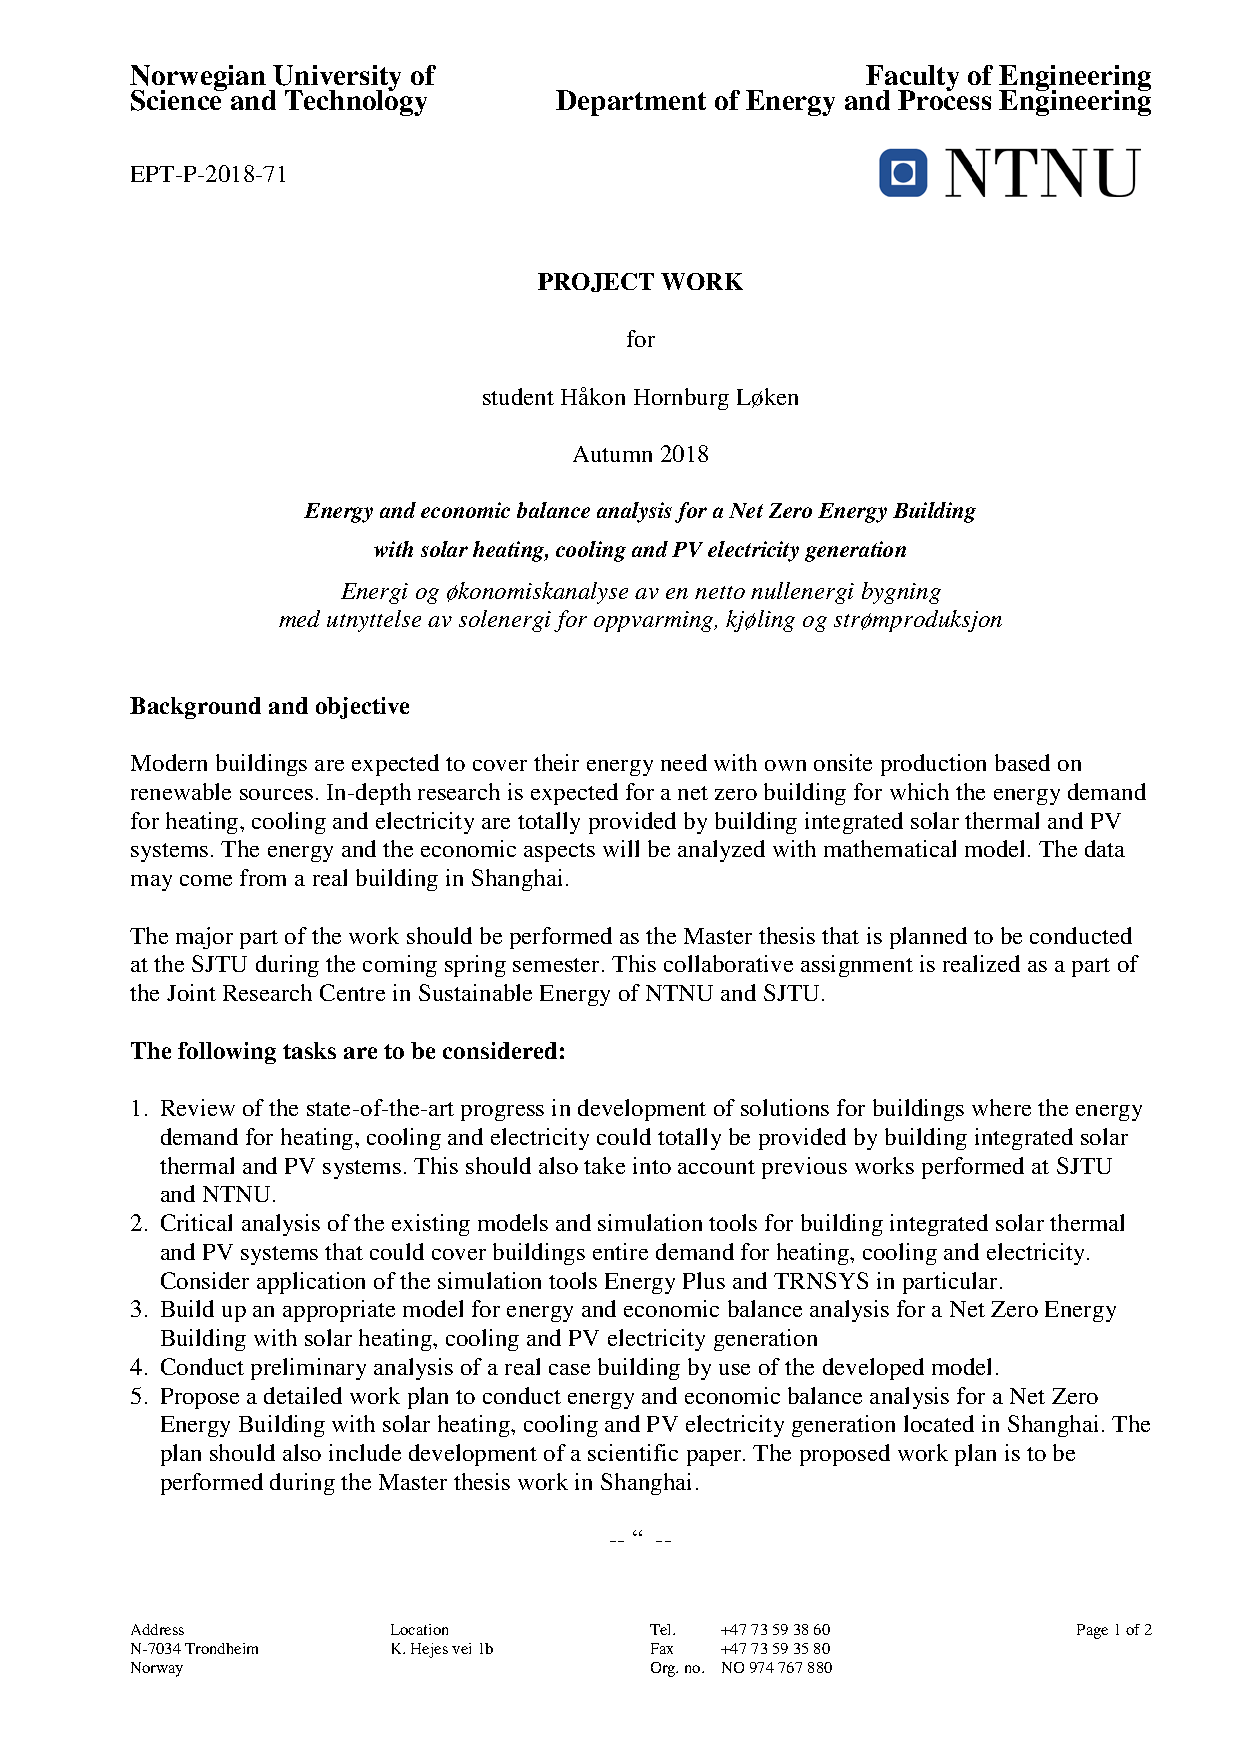
\includepdf[pages={1}, pagecommand={}]{vedlegg/oppgside1.pdf}
\clearpage
\pagestyle{empty} %No headings for the first pages.

\includepdf[pages={1}, pagecommand={}]{vedlegg/oppgside2.pdf}
\clearpage

\pagenumbering{roman}

% 
\chapter*{Preface}
This report is the product of TEP4530 - Energy and Indoor Environment, Specialization Project at Norwegian University of Science and Technology (NTNU), and counts for 15 credit points. The assignment is realized as a part of the Joint Resarch Centre in Sustainable Energy of NTNU and Shanghai Jiao Tong University (SJTU). The report is written for the Department of Energy and Process Engineering, NTNU. Main supervisor has been Professor Vojislav Novakovic and  Co-Supervisor has been Prof. Yanjun DAI. The work is planned to be continued as a master thesis, conducted at SJTU, spring 2019. \\
\\
The main motivation for this project was the interest of contributing to a sustainable future by investigating the possibility of profitable net Zero Energy Buildings.  This interest comes from various courses given at NTNU, and information obtained from school from young age.  \\
\vspace{4cm}
\\
18.11.2018, Trondheim \hfill 
\includegraphics[]{vedlegg/uskrift.png} \\
\noindent\rule{5cm}{0.4pt} \hfill \noindent\rule{5cm}{0.4pt} \\
Date, Place \hfill Håkon H. Løken \hspace{2.35cm} \\
\vfill
\begin{center}

\includegraphics[scale=0.35]{vedlegg/logo.png}
\end{center}

\newpage

%
\chapter*{Acknowledgments}
I would like to thank the Department of Energy and Process Engineering at the faculty of engineering at NTNU. The courses taught by the department, by the professors connected to it, has given me the knowledge that made it possible to complete this work. I want to thank especially my supervisor, professor Vojislav Novakovic for guiding my in this project, and also for teaching me in courses connected to this topic. The courses has developed my interest in the field of study and is the main reason for conducting this work. I also want to thank Professor Hans Martin Mathisen, Professor Guangyu Cao, Associate Professor Laurent Georges, Associate Professor Natasa Nord and Associate Professor Mohamed Hamdy for teaching and providing help when needed. \\
\\
I would like to thank the Department of Energy and Process Engineering for providing a great study environment with an open office study room at "Varmetekniske laboratorier". The room has been optimal as it is always a free desk, an additional computer screen for each student and storage possibilities. It has also been great to study in a room with so many student that has knowledge on the same topic. The close access to the professors and other people working for the department has also been great. Finally I want to thank the department for the  supply of coffee. It was especially appreciated at early mornings and long nights working.
\newpage

\chapter*{Abstract}
The abstract should be short, preferably no more than one standard A4 page, and give a short overview of the contents of your text. You should tell the reader:

% - what you investigated
% - how you did it
% - what you found out
% By reading the abstract, the reader should be able to determine whether or not they are interested in reading the rest of your paper.


\newpage

\chapter*{Sammendrag}


\newpage

\tableofcontents %Table of contents 

\listoffigures
 
\listoftables

\setlength{\parindent}{0em}
\setlength{\parskip}{1em}
\pagestyle{plain} 

\cleardoublepage
\pagenumbering{arabic}

\chapter{Introduction}
% present what we already know, and what we do not know yet know about the subject. You do this by presenting:

% - A problem or phenomenon you want to study
This research will analyze the energy demand of a modern building, located in Shanghai, China, and investigate the possibility of covering the entire energy demand by solar heating, cooling and PV electricity. An economic analysis will be made to determine whether a project like this is profitable.
% - The reasoning behind your choice of topic
\begin{wrapfigure}{o}{0.5\textwidth}
    \centering
    \vspace{3mm}
    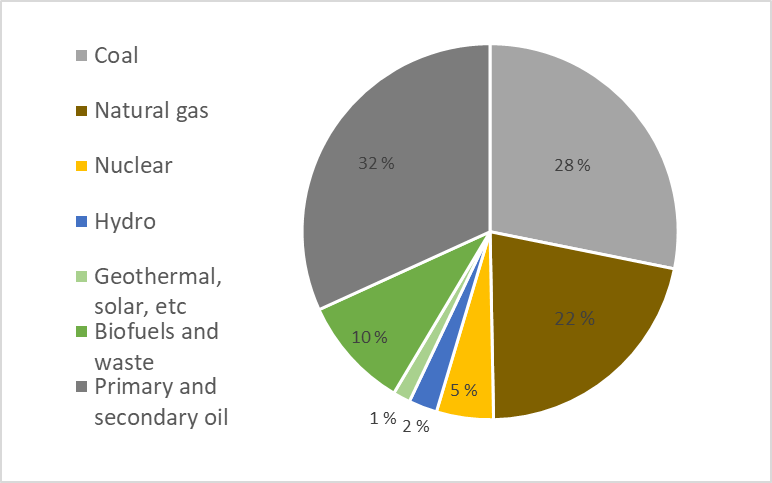
\includegraphics[width=0.45\textwidth]{vedlegg/TPESnew}
    \caption{\textit{Total primary energy supply by source, 2015}}
     \vspace{-6mm}
    \label{fig:TPES}
\end{wrapfigure}

The reason behind this topic is based on global warming, perhaps the greatest challenge the world has ever faced. The global primary energy consumption was in 2015, 13 669 million tonnes of oil equivalent (\ac{Mtoe}), and from figure \ref{fig:TPES}, it can be seen that 81.5\% of that came from the fossil fuels coal, natural gas and oil \cite{stats}. Energy production from fossil fuels results in emissions of the greenhouse gas carbon dioxide (\ac{co2}), and as a consequence of this the concentration of the gas in the atmosphere has increased approximately 1\% yearly from 338.89 ppm in 1980 to 404.97 in 2017 \cite{co2levels}. A graphical representation of CO$_2$ concentration in the atmosphere from 1980 to 2017 is displaced in figure \ref{fig:co2}. 

In the same time period the global average temperature, illustrated in figure \ref{fig:temp}, has increased with 0.63$^\circ$C, and was in 2016 a record high 0.99$^\circ$C above pre-industrial levels \cite{temp}. The global temperature depends on many factors, but a connection between the concentration of CO$_2$ in the atmosphere and the global mean temperature is beyond doubt. As the concentration of CO$_2$ continues to rise, the temperature on the planet is expected to do the same. 

\begin{wrapfigure}{i}{0.5\textwidth}
    \centering
    \vspace{-4mm}
    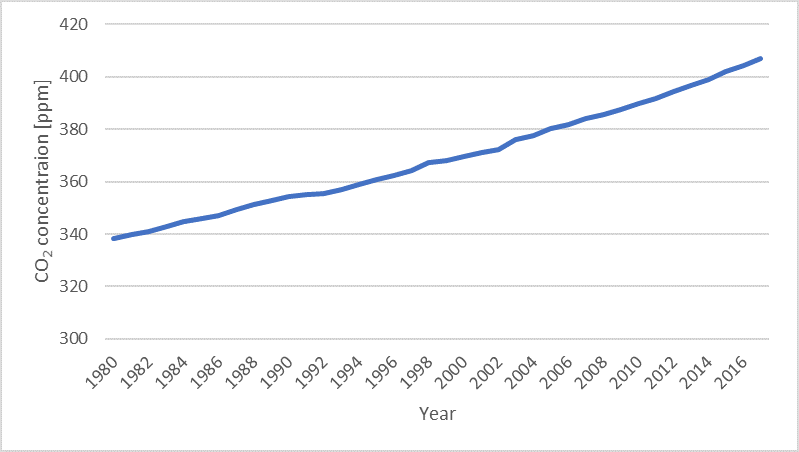
\includegraphics[width=0.4\textwidth]{vedlegg/co2new}
  \caption{\textit{CO$_2$ concentration in the atmosphere from 1980 - 2017}}
  \label{fig:co2}
  \vspace{-30mm}
\end{wrapfigure}


The Paris Agreement on climate change is an agreement signed by more than 190 countries, and a central aim is to reduce the damage of global warming to less than 1.5$^\circ$C rise of global mean temperature compared to pre-industrial levels \cite{paris}. 


\pagebreak

\begin{wrapfigure}{o}{0.4\textwidth}
    \centering
    %\vspace{-4mm}
    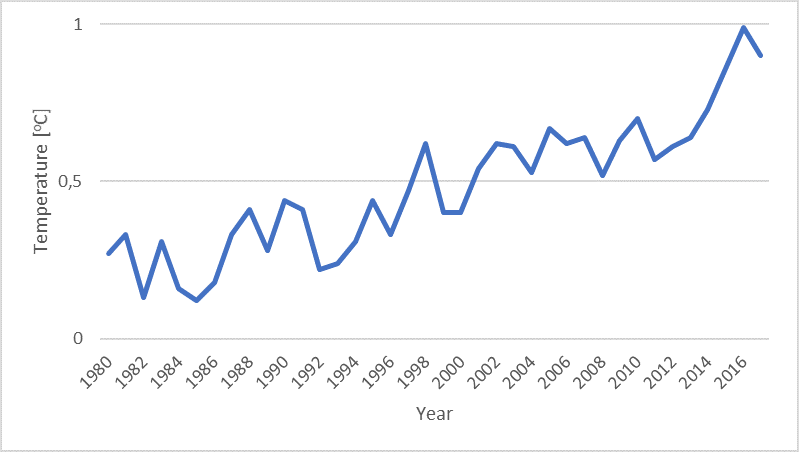
\includegraphics[width=0.4\textwidth]{vedlegg/tempnew}
    \caption{\textit{Global mean temperature from 1980 - 2017, compared to pre-industrial levels}}
    \label{fig:temp}
\end{wrapfigure}

An Intergovernmental Panel on Climate Change (IPCC) special report on the impacts of global warming states that emission of greenhouse gases needs to be reduced by 45\% compared to 2010 by 2030 in order to achieve the goal of the Paris agreement, and there are four main approaches to obtain that goal \cite{Ipcc}. The first and most effective is reducing the energy demand. The second is to replace energy produced by fossil fuels with energy from renewable sources. Solar-, hydro-, wind- and wave energy are examples of energy sources that are renewable. The third approach is to make energy production from fossil fuels more efficient. It is not realistic to cover the  entire global energy demand by renewable sources within 2030, so its important to make use of the energy from fossil fuels most efficient to reduce emissions of greenhouse gases. The last approach is to capture and store greenhouse gases such as CO$_2$ and methane to reduce the levels of the gases in the atmosphere. This report is focusing on the first two approaches as they are most relevant to this topic.

\begin{wrapfigure}{o}{0.5\textwidth}
    \centering
    \vspace{-4mm}
    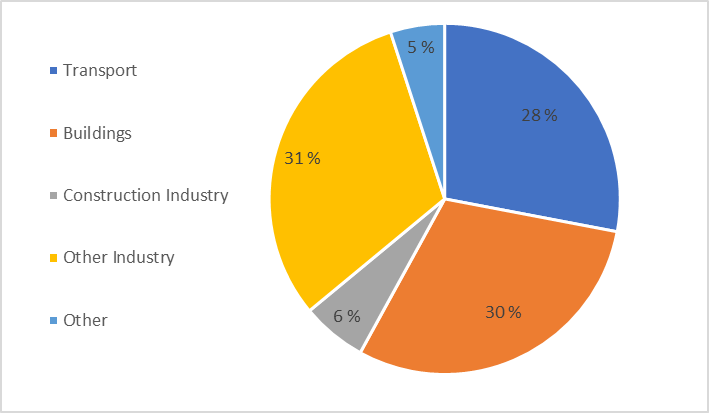
\includegraphics[width=0.5\textwidth]{vedlegg/sec}
    \caption{\textit{Global final energy consumption by sector, 2015}}
    \label{fig:sector}
    \vspace{-4mm}
\end{wrapfigure}

The consequences of a rise in global mean temperature is more extreme weather, drought, floods, rise in sea level because of melting polar ice, which again will lead to areas located at sea level today, under water in the future. The magnitude of this effect all depends on how much the temperature increases, and the difference between 1.5 and 2 or even 3 degrees above pre-industrial levels are severe \cite{Ipcc}. 

The operation of buildings is responsible for 30\% of final energy consumption and more than 55\% of electricity demand globally \cite{ETP}. To accomplish the target of the Paris Agreement, the building sector therefore clearly has a huge responsibility. The energy demand of buildings in the future has to decrease and at the same time produce on site renewable energy.

% - The research question or hypothesis you set out to investigate
This report will analyze the energy consumption of a net Zero Energy Building located in Shanghai, China, with integrated solar thermal and PV systems for cooling, heating, and electricity production. There will be made an economic analysis of the project, and recommendation for further work.
% Towards the end of the introduction, you should also say something about how your text is structured, as a short guide to the reader.

The thesis will first explain the theory behind the technology that is being investigated, before the methodology of the research will be described. Then the development of the model used for energy simulations will be explained and different simulation tools will be discussed. The results of the simulation will then be presented, analyzed and discussed before a conclusion will be drawn. The thesis will end with a plan for further work. 

\chapter{Theoretical background}
In this chapter the different terminologies used in this report will be introduced and the importance in context to this research will be discussed. 

\section{Energy management in buildings}
\begin{wrapfigure}{o}{0.5\textwidth}
    \centering
    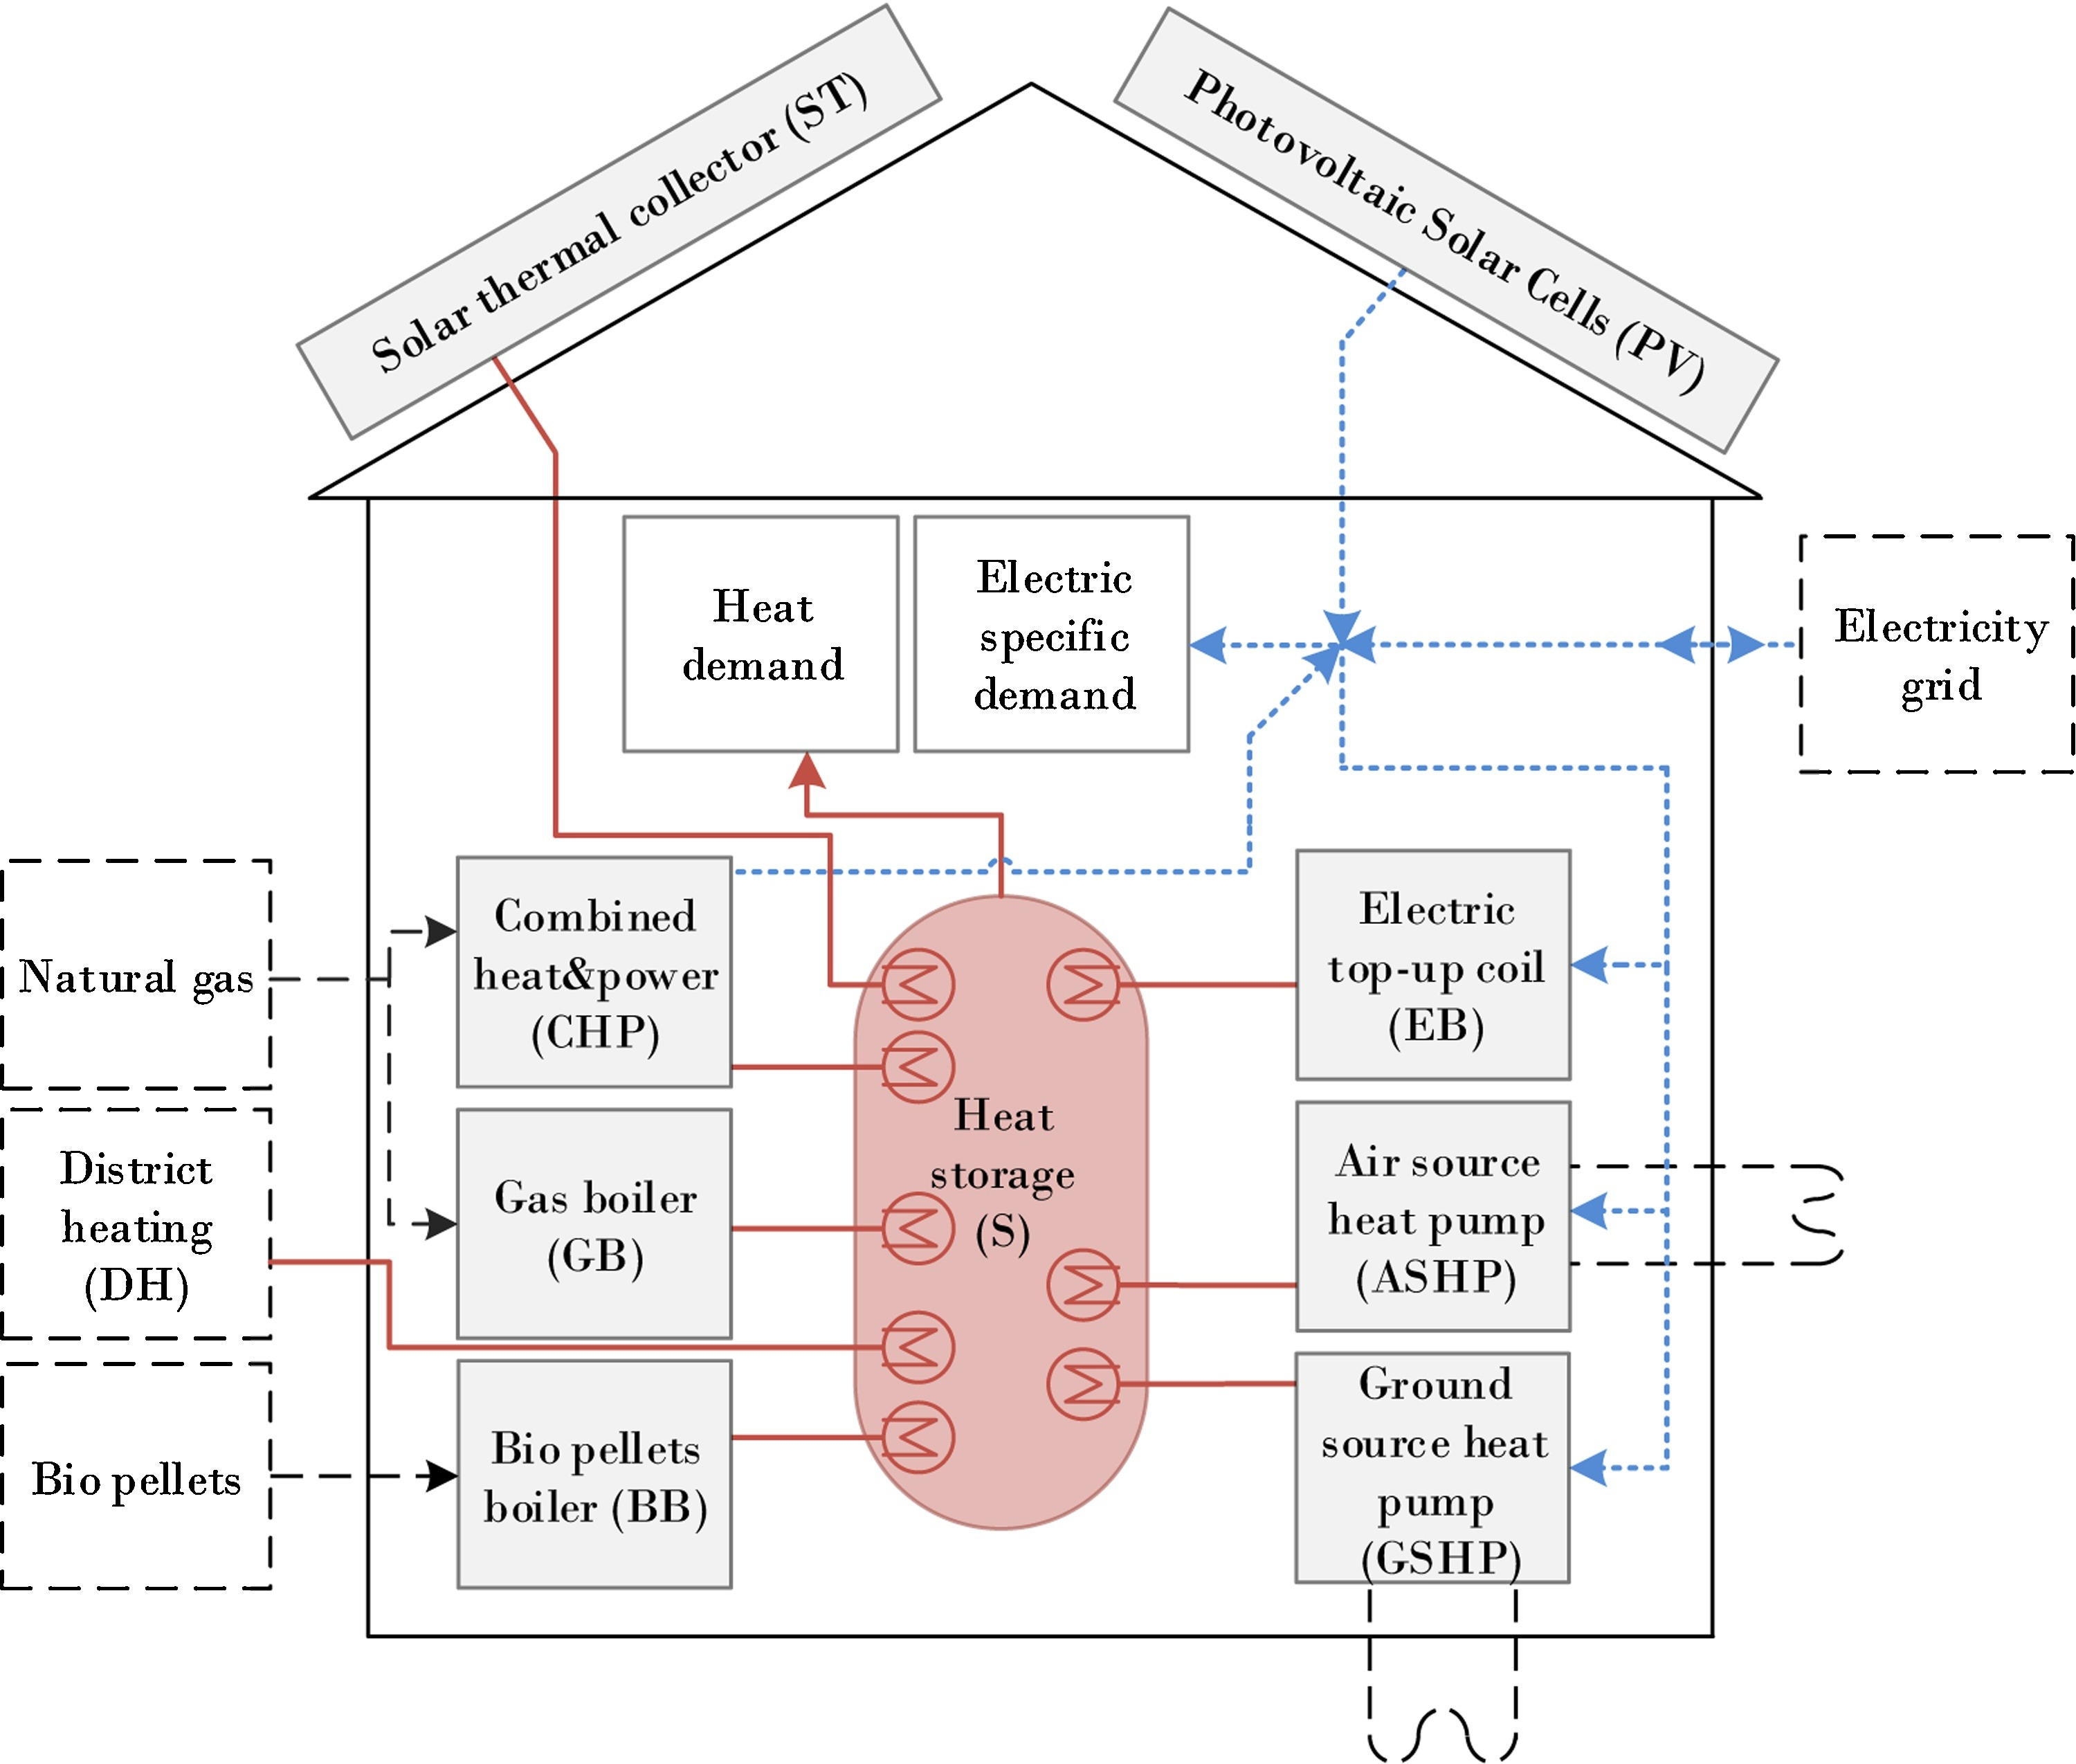
\includegraphics[width=0.45\textwidth]{vedlegg/grid.jpg}
    \caption{\textit{An example of a building, including building installations with connection to electricity grid}}
    \label{fig:gridl}
\end{wrapfigure}

A building is defined as a permanent or temporary structure enclosed by a building envelope, including building installations. The main purpose for a building is to give protection against external climate and disturbances. The buildings also need to provide a healthy and comfortable indoor environment without causing unreasonable high expenses in regards of investment and operational costs of the building. Net Zero Energy Buildings (\ac{nzeb}s) are buildings that aim to minimize the environmental impact by reducing the energy demand and producing on site renewable energy that compensates for the energy demand. The term net is used to refer to that the building is connected to the energy infrastructure and underlines the fact that there is a balance between energy taken from and supplied back to the energy grid over a period of time. An illustration of a building including an example of building installations is displayed in figure \ref{fig:gridl}.

The energy consumption of a building is affected by the external climate, the building envelope, technical installations, operation and maintenance. The operation and maintenance is depending on the occupant behaviour and wanted indoor environmental conditions and are referred to as human influenced factors. External climate, the building envelope and building installations are, unlike the human influenced factors, factors that can not be controlled. 
\pagebreak

\begin{wrapfigure}{i}{0.5\textwidth}
    \centering
   %\vspace{1mm}
    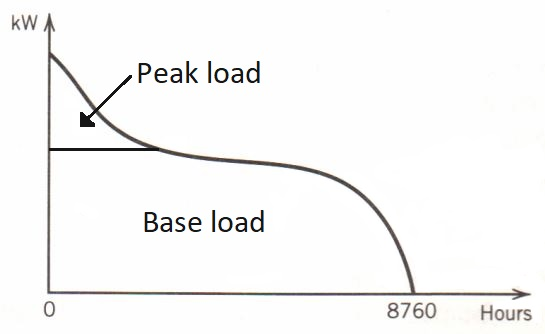
\includegraphics[width=0.5\textwidth]{vedlegg/loaddur}
    \caption{Load duration curve over a year}
    %\vspace{18mm}
    \label{fig:ldc}
\end{wrapfigure}

The energy consumption of a building is defined by the energy need for space heating and cooling, ventilation, domestic hot water, lighting and equipment. Internal- and solar gains are also taken into account when calculating energy demand. To design the optimal solution for each building, a load duration curve should be used to ensure correct sizing of the HVAC components. A load duration curve, illustrated in figure \ref{fig:ldc}, is an estimation of total energy demand over a year and describes the size and duration of different heat or cooling demands. A system with low operation cost should be installed to cover the base load which could cover between 90-95\% of total energy demand. The reason its not desirable to cover the entire energy demand is the high investment cost for the effect needed, so a system with a low investment cost should therefore be installed to cover the peak load, even though it has a higher operation cost. 
%An air tight envelope with low heat transfer coefficient (U-value) in the building materials ensures a low energy demanding building.

\section{Heat transfer}
\begin{wrapfigure}{0}{0.5\textwidth}
    \centering
   \vspace{5mm}
    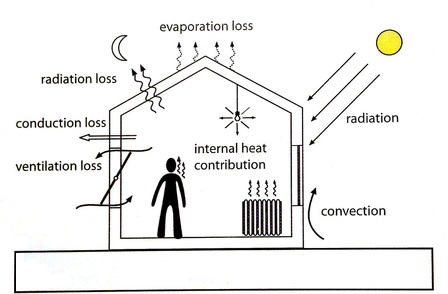
\includegraphics[width=0.5\textwidth]{vedlegg/7281185.jpg}
    \caption{Heat balance in a building \cite{dahl}.}
    \label{fig:ccr}
\end{wrapfigure}

Heat is transferred through either conduction, convection, radiation or evaporation. In practice in a building it is a combination of conduction, convection and radiation. 

The heat balance of the building is illustrated in figure \ref{fig:ccr} with the different parameters that has an influence on the heat transfer. It is the thermal transmittance of the building envelope, also known as U-value, that decides how much heat that is transferred through the building. The better a building is insulated, the lower the U-value is and less heat is transferred through the envelope. To calculate the U-value, the thermal resistance, R, needs to be calculated in each layer. The R-value through construction materials is found by dividing the thickness (t) by the thermal conductivity ($\lambda$) of the material as shown in equation \ref{eq:R}. 

\begin{equation}
    R = \frac{t}{\lambda} \hspace{5mm} [K m^2/W]
    \label{eq:R}
\end{equation}

The U-value is calculated using equation \ref{eq:U}.

\begin{equation}
    \label{eq:U}
    U = \frac{1}{\sum R} \hspace{5mm} [W/m^2 K]
\end{equation}

The U-value alone does not describe all of the heat loss because thermal bridges appear typically in connection points between constructions. This is parts where the thermal resistance is significantly lower than rest of the construction and the heat loss is higher. This needs to be taken into account, and prevented as much as possible. 

\begin{equation}
    Q = U \cdot A \cdot \Delta T [W]
\end{equation}

\section{Indoor Environment and Thermal Comfort}
A study done in 2001 showed that people spent in average almost 87\% of their life inside buildings, either at home or at work \cite{Nhaps}. It is therefore obvious that the indoor environment has an enormous impact on human health and well being. Productivity is related to the ability to perform various tasks and studies have shown a clear connection between productivity and indoor environment. The noise level, temperature and perceived air quality are all parameters that has an effect on the productivity level. Studies have shown that people perform tasks more accurately, faster and over a longer time with increased productivity. Other consequences are that people feel healthier, sustain stress more effectively and enjoy spending time at work. Less sick leave and improved performance is very economically beneficial for a company.
Indoor environment can be defined as a composite of the five elements; Thermal-, atmospheric-, acoustic-, actinic-, and mechanical environment. The acoustic and mechanical environment has no impact on the energy use or operation costs and will not be discussed further in this report.

The thermal environment depends on the indoor air temperature, surface temperatures, temperature gradients, relative humidity and air velocity. The thermal comfort is defined as 'that condition of mind which expresses satisfaction with the thermal environment' (NS-EN ISO 7730), and depends also on the clothing level and activity level. Clothing level describes the thermal resistance between the surface of the skin and the outer surface of the clothing, with the unit clo. Activity level is a measure of the metabolic rate from energy production by the human body with the unit met. Clothing level is assumed to be equal to 1 clo in the winter and 0.5 clo in the summer. Sedentary activities like office work is equal to 1.2 met. 

$$ 1.0 \hspace{1mm} \mbox{clo} = 0.155 \hspace{1mm} m^2K/W$$
$$ 1.0 \hspace{1mm} \mbox{met} = 58 \hspace{1mm} W/m^2 $$

\begin{wrapfigure}{0}{0.45\textwidth}
    \centering
    \vspace{-4mm}
    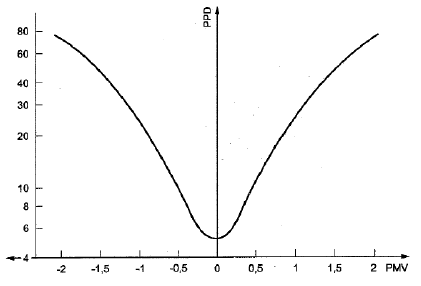
\includegraphics[width=0.4\textwidth]{vedlegg/pmvppd.png}
    \caption{Relation between PMV and PPD}
    \label{fig:my_label}
 \end{wrapfigure}
 
Thermal comfort is an individual perception and it is therefore difficult to make everyone in a room completely satisfied. Predicted Mean Vote (\ac{pmv}) is a psycophysic 7-point scale from -3, cold, to +3, hot where 0 corresponds to thermal neutral, that can be calculated for a given situation. Predicted Percentage of Dissatisfied (\ac{PPD}) can be derived from PMV and is the predicted percent of dissatisfied people at each PMV. The aim is to reach category A, a PPD of 6\% or less. 
%\pagebreak

Figure \ref{fig:opt} shows the optimum operative temperature in category A for different activity and clothing levels. Clothing level 1 clo and activity level 1.2 met gives and optimum operative temperature of 21.5$^o$C $\pm$ 1$^o$C. Operative temperature (\ac{To}) is defined as "the uniform temperature of an imaginary black enclosure in which an occupant would exchange the same amount of heat by radiation and convection as in the actual non-uniform environment(ISO 7730:2005). With metabolic rates between 1.0 and 1.3 and air velocities below 0.10 m/s, operative temperature can be calculated using equation \ref{eq:to}. 

\begin{figure}[h!]
    \centering
    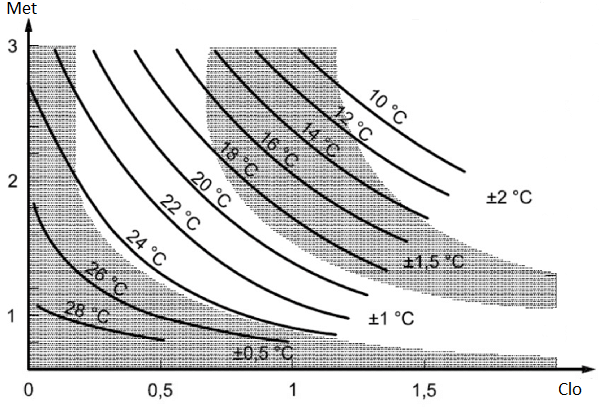
\includegraphics[scale=0.6]{vedlegg/opt.png}
    \caption{Optimum operative temperature category A.}
    \label{fig:opt}
\end{figure}

\begin{equation}\label{eq:to}
    t_o = \frac{(t_a+t_{mr})}{2}
\end{equation}

where,

$t_a$ \hspace{1mm} = Air temperature [$^o$C] \\
$t_{mr}$ = Mean radiant temperature [$^o$C] \\




\begin{table}[h!]
    \centering
        \caption{Design criteria for office building, activity level: 1.2 met, Clothing level: 0.5 clo summer, 1.0 clo winter, category A (ISO 7730).}
        \arrayrulecolor{white}
    \begin{tabular}{p{3.5cm}|p{1.8cm}|p{1.8cm}}
    \rowcolor{denim} \color{white} Parameter & & \\
    \hline
       \rowcolor{lblue} & Summer & Winter  \\
         \hline
         \rowcolor{denim} Operative temp [$^o$C] & 24.5 $\pm$ 1.0 & 22.0 $\pm$ 1.0  \\
    \hline
       \rowcolor{lblue} Relative humidity [\%] & 60 & 40  \\
         \hline
         & &  \\
    \end{tabular}
    \label{tab:design}
    \arrayrulecolor{black}
\end{table}

Atmospheric environment indicates the perceived indoor air quality and depends on the concentration of air pollutants in the indoor air, amount of particles and smell. Ventilation is used to provide good indoor air quality by supplying fresh air and extracting contaminated air. The ventilation rate should be based on pollution load from occupants and materials. Concentration of CO$_2$ is a common way to control the quality of the air. The gas is not toxic for humans at low levels but gives a good indication of how good the air change in a room is. 

Actinic environment is an indication of the quality of light inside the building and is described by the daylight factor. The daylight factor represent the amount of illumination available indoors relative to the illumination present outdoors at the same time under overcast skies.

To obtain good indoor climate, a heating, cooling and ventilation system might be required to be installed, depending on the location and use of the building.



\section{Building Installations}
Building installations include all attached and fixed installations connected to a building. That includes systems for heating, cooling, ventilation and sanitary, which has the collective term HVAC systems. It is also consisting of all electrical and gas installations, fire alarms and fire extinguishing installations and access and intruder control. This research will focus on the systems for space heating and cooling, heating of domestic hot water, photovoltaic panels for electricity production, ventilation system and lighting as they are most relevant for an energy analysis.

\subsection*{Space Heating and Cooling}
A heating system for space heating and heating of domestic hot water will be installed to provide the desired temperatures. A heat pump will be installed to cover the base load for heating. The same heat pump will be used to cover the cooling load. 

\subsection*{Heat Pump}
A Heat Pump (\ac{hp}) is a system that reduces the primary energy use by utilizing renewable energy and can be used for heating and cooling purposes. There exists many different types of heat pumps, with different working fluids, but they are all based on the same main function. The heat pump consists of four main components including a compressor, a condenser, an expansion valve and an evaporator. The evaporator extracts heat from a heat source and transfer the heat to a working fluid. The working fluid transfers thermal energy to the supply system by changing state throughout a continuous cycle driven by the compressor. A simple sketch is shown in figure \ref{fig:HP} to illustrate the principle behind the heat pump.

\begin{figure}[h!]
    \centering
    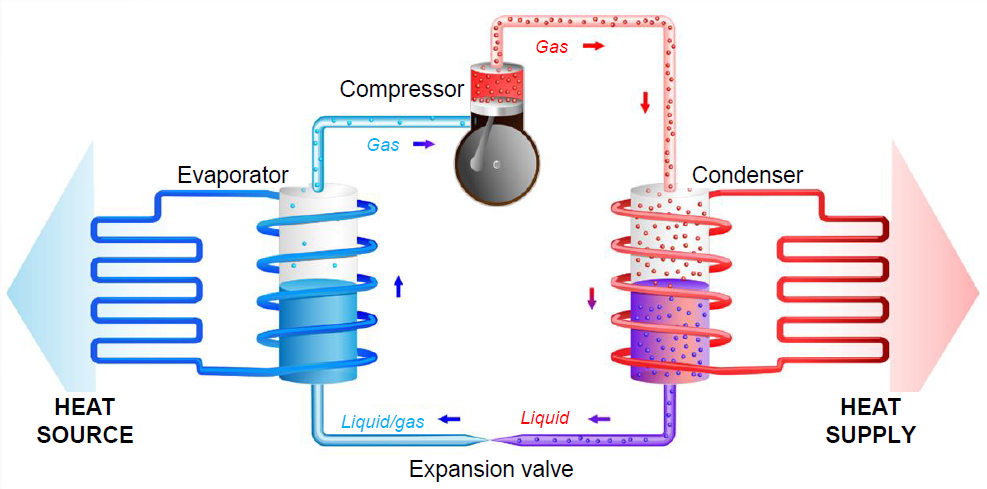
\includegraphics[scale=0.35]{vedlegg/HP.png}
    \caption{Heat pump cycle}
    \label{fig:HP}
\end{figure}

A heat pump has typically a coefficient of performance (\ac{COP}) of between 2 and 5, depending on the type, which means it can reduce the energy demand for space heating and cooling by between 50-80\%. The energy saving can be calculated by using equation \ref{eq:ES}.

\begin{equation}
    \mbox{Energy saved} = 1 - \frac{1}{COP} [\%]
    \label{eq:ES}
\end{equation}

The \ac{COP} can be calculated using equation \ref{eqn:COP} where Q is the delivered heat, and W the necessary work done by the compressor. A heat pump that can deliver a big amount of heat is however often expensive to install so it is therefore beneficial to use to cover the base load for heating and cooling. Primary energy use when using a heat pump can be calculated using equation \ref{eqn:PEU}.

\begin{equation} \label{eqn:COP}
    \mbox{COP} = \frac{\ac{Q}}{\ac{W}}
\end{equation}

\begin{equation}\label{eqn:PEU}
    \mbox{Primary energy use} = \mbox{energy coverage} \cdot \frac{\mbox{Heat demand}}{COP}
\end{equation}

\begin{wrapfigure}{0}{0.35\textwidth}
    \centering
    %\vspace{-4mm}
    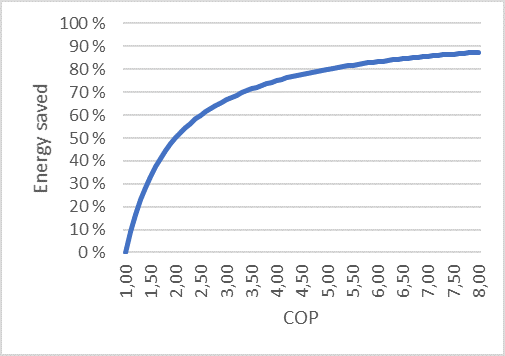
\includegraphics[width=0.35\textwidth]{vedlegg/cop1.png}
    \caption{Relationship between COP and energy savings}
    \label{fig:c}
 \end{wrapfigure}
 
Heat pumps can utilize different types of renewable energy depending on the location and availability of resources. Different sources are ground, ground water, sea water, gray water, sewage and air. Air source is the only source that are available everywhere, and is the one that will be used and discussed in this report. 

\subsubsection*{Air Source Heat Pump (\ac{ASHP})}
Ambient air is the most available heat source for use in a heat pump, has the lowest installation costs and are for those reasons among the most commonly used in heat pumps. A similar heat source is exhaust air from the ventilation system, which has a slightly higher investment cost, but a lower operation cost and maintenance need. Exhaust air also has a more steady, reliable temperature than ambient air. The exhaust air is believed to be the optimal solution for heat source. A air to water heat pump will be used.

\subsection*{Heating system}
Water born heating system

\section{Solar Energy}
For the building to qualify as a \ac{nzeb} it needs to produce on site renewable energy equal to, or greater than, the primary energy use. Solar energy is an important source of renewable energy, and has a potential greater than the total world energy demand. It is however demanding to utilize more than a fraction of that incoming energy. Solar energy can be utilized in the shape of thermal energy by direct solar gains, or by solar thermal collectors. Solar energy can also be converted into electricity by photovoltaics (\ac{pv}), or applied directly as daylight. Solar energy is utilized by transforming solar radiation into heat and electricity and consists of a transformer unit, a distribution system and an energy storage unit. How much energy it is possible to extract depends on solar irradiation and angle of the panels

\subsection{Photovoltaics}
Electricity is generated from solar energy by transforming radiation into electricity using photovoltaic cells before storing the generated power in batteries. The electricity produced can be used directly on site or exported and sold back to the grid depending on the need. \ac{pv} panels produces and stores direct current (DC) electricity which needs to converted by an inverter to an alternating current (AC) used on the grid. Modules commercially available today has an efficiency in the range 15\% to 20\% of irradiation, and can be installed on the outside of the building envelope. This report will investigate how many modules that will be needed to cover the entire demand and what the cost will be. 

\subsection{Solar thermal collector}
Solar thermal collectors are used for space heating or heating of hot water and the efficiency is in the range 40-70\% of irradiation. 

\section{Ventilation system}
The purpose of a ventilation system is to provide good indoor air quality by removing pollutants and odors. This can be achieved by natural forces like wind and pressure difference or by mechanical forces. It is also possible to combine the two methods. The use of natural forces are the most economical in terms of installation cost and operational costs but is very limited in controlling the indoor environment. An office has a high demand for good air quality for good productivity and reducing the risks of sickness. To obtain desired indoor environment a mechanical ventilation system is therefore preferred.

The most common mechanical ventilation methods are mixed and displacement ventilation. Mixed ventilation is based on the principle that all air inside a room is completely mixed with a uniform temperature and pollutant concentration. Fresh air is supplied into the room at high velocities to make that happen. In displacement ventilation utilizes buoyancy forces as colder air is supplied close to the floor before heated up by pollutant sources, rising, bringing contaminants away from the occupied zone before exiting the room close to the ceiling. Displacement ventilation is preferable to use in large rooms with high heat loads. One disadvantage of displacement ventilation is the risk of draft from supplying cold air into the occupied zone. Mixed ventilation is believed to be a better option for the office building

The ventilated air can be supplied and extracted at a constant air volume (\ac{CAV}) or with a variable air volume (\ac{VAV}) with the use of demand controlled ventilation (\ac{DCV}). DCV can use temperature, occupancy or CO$_2$ concentration sensors to decide how much fresh air the ventilation system should provide to maintain good indoor air quality. DCV is a more complex system that has a higher investment cost, but can be cheaper and more accurate in operation. CAV is not as flexible as DCV but also has the possibility of supplying air at different rates according to predefined schedules. The weekly schedule is predefined for the office building.

The chosen ventilation system for the building is mechanical, mixed ventilation with a CAV. There can also be installed a manual solution to extend ventilation time at times when it is needed.

A heating and a cooling battery will also be installed in the air handling unit (\ac{AHU}) will also be installed for the purpose of heating and cooling the ventilated air. A heat recovery unit extracts heat from the exhaust air to preheat the supply air, and should be installed to save energy. There are two different types of heat recovery units. A regenerative heat exchanger that 

\section{Lighting}


\section{Building automation}
Building automation is the concept of controlling the building systems according to schedules to reduce energy. The main purpose is to provide the right amount of heating, cooling, ventilated air and lighting when people are present in the building. 

\section{Economics}
Renewable, on site energy is only of interest for a company if the project is more profitable than the alternative conventional energy. The profitability depends on the investment costs (\ac{investment}), the life time (\ac{lifetime}) of the components and yearly savings (\ac{balance}) compared to the alternative. A net present value (\ac{npv}) tells if the investment is better than the alternative of investing the money in something different. Net present value can be calculated using equation \ref{eq:npv}, where \ac{realrate} is the real rate of return which expresses the return the company believe the money can get when invested somewhere else. 

\begin{equation}
    NPV = -I + \sum_1^n \frac{B_t}{(1+r)^t}
    \label{eq:npv}
\end{equation}

Energy prices are difficult to predict, so future energy prices are assumed to follow the development of historical prices. All energy demand is assumed covered by electricity for simplicity. 

\chapter{Methodology}
In this chapter the research methods used in this project will be described, explained and discussed. The mathematical models that has been used to analyze the energy and economic aspect will be presented. 

\section{Building Performance Simulation}

Building performance simulation is a computer based, multidisciplinary, and problem oriented mathematical model of a given aspect of building performance based on fundamental physical principles and engineering models. It assumes dynamic boundary conditions and is normally based on numerical methods that aim to provide a simplified and approximate solution of a phenomenon or object of the real world. It will be adopted in this research to estimate the behaviour of a real building located in Shanghai, China to improve the design and operation. Many different simulation tools exists and they variate in system layouts and degree of details in their approach. EnergyPlus and TRNSYS will be used and discussed in this report.

\subsection{TRNSYS}
Transient Systems Simulation Program (\ac{TRNSYS}) is based on a system layout that allows you to build the system from components in a library. It uses a (black box) approach which is based on experimental data.

\subsection{EnergyPlus}

\begin{wrapfigure}{0}{0.3\textwidth}
    \centering
    \vspace{-6mm}
    
\includegraphics[width=0.2\textwidth]{vedlegg/e+.png}
    \caption{EnergyPlus logo}
    \vspace{-5mm}
    \label{fig:e+}
 \end{wrapfigure}
 
EnergyPlus is a whole building energy simulation program used to model both energy consumption—for heating, cooling, ventilation, lighting and plug and process loads—and water use in buildings. EnergyPlus is funded by the U.S. Department of Energy’s (DOE) Building Technologies Office (BTO), and managed by the National Renewable Energy Laboratory (NREL). The program is available for free download for non commercial individual and educational use \cite{energyplus}.

The software calculates the heating and cooling load necessary depending on the description of the building envelope, technical installations and associated weather data file. 

EnergyPlus lacks a user friendly interface and it is therefore quite time consuming to learn to use the program. Sketchup was used to design the building geometry, and the thermal zones in the building. The material data was then later edited in Open Studio, where also technical installations were added to the building. Energy simulations was made in EnergyPlus. 

\section{Data collection}
The geometry and use of the building was assumed to represent a typical small office building. Design criteria from Chinese government was used to decide heat transfer coefficients for the building envelope to make sure the building met all legal requirements. These values has been implemented in the simulation models, together with default values set it the programs. This simplification was made as no other data was available and it describes well a typical office building, without any huge investments on the building envelope made to make it energy efficient. This may lead to the result being a worst case scenario and a real case to have the same or a lower energy demand. 

The energy demand is based on simulation in EnergyPlus, where the whole building geometry has been simulated in combination with a HVAC system. This energy demand is beeing used as basis for TRNSYS simulation, where a model combined of HVAC, domestic hot water, heat pump and solar thermal energy was build to calculate if the system can meet the energy demand. Solar energy was also simulated in EnergyPlus to 
% How did I collect the data
% How did I interpret the data collected
% How did I choose these methods?
% Strengths and weaknesses of these methods

\chapter{Model}
This chapter describes in detail the building that is analyzed, the purpose of the building, the technical installations and assumptions and simplifications that are made for the model used in energy simulations.

\section{Location and Climate}
The building analyzed is located in Shanghai, China. At an latitude of 31.17$^o$ N and longitude of 121.43 $^o$ E it is in the category "hot summer and cold winter zone" according to Chinese regulations. That means there is a big demand for heating in the winter months, and for cooling in the summer months. Relative humidity is high in the region and dehumidification needs to be considered. 

\begin{figure}[h!]
    \centering
    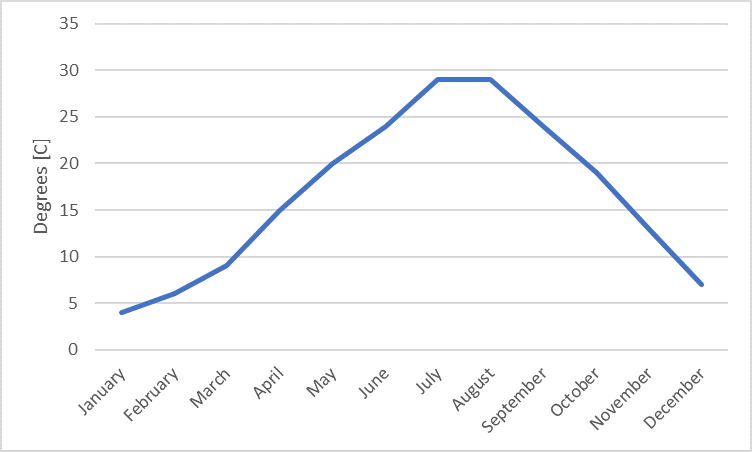
\includegraphics[scale=0.6]{vedlegg/tem.png}
    \caption{Average temperatures in Shanghai by month \cite{temp}.}
    \label{fig:temp}
\end{figure}

\subsection*{Governmental Requirements}
There are many factors influencing the energy demand of a building. For simplification the main focus is on the heat transfer coefficient or U-value of the building envelope. The authorities in China has design standards for u-values according to what climate zone the building is located, and the most relevant values is displayed in table \ref{tab:uvalue}. 

\begin{table}[h!]

    \centering
        \caption{U-value requirements for new commercial buildings in hot summer cold winter climate zone, China. \cite{uvalue}}
    \begin{tabular}{|p{1.5cm}|p{1cm}|}
         \hline
         \multicolumn{2}{|c|} {\textbf{U-value (W/m$^2$K)}} \\
         \hline
         \textbf{Roof} & 0.7 \\
         \hline
         \textbf{Wall} & 1\\
         \hline
         \textbf{Floor} & 1 \\
         \hline
         \textbf{Window} & 2.5\\
         \hline
         \textbf{Other} & 3\\
         \hline
    \end{tabular}

    \label{tab:uvalue}
\end{table}


\section{The Building}
The building is a 1 story, commercial, office building with a total of 420m$^2$. It consists of one closed office, one conference room, one open office room, one mechanical room, a break room and two restrooms. The building geometry is illustrated in figure \ref{fig:zones} where the different construction materials between interior and exterior walls can be seen.

\begin{table}[h!]
    \centering
        \caption{Caption}
    \begin{tabular}{|c|c|c|}
    \hline
    Space & Geometry & Area \\
    \hline
        Closed Office & 6m $\cdot$ 6m & 36m$^2$  \\
        \hline
        Conference Room & 6m $\cdot$ 12m & 72m$^2$  \\
    \hline
    Open Office & 10m $\cdot$ 20m + 2m $\cdot$ 2m & 204m$^2$ \\
    \hline
    Mechanical Room & 3m $\cdot$ 6m & 18m$^2$ \\
    \hline
    Break Room & 9m $\cdot$ 6m & 54m$^2$ \\
    \hline
    Restrooms & 2 $\cdot$ 3m $\cdot$ 6m & 36m$^2$ \\
    \hline
    Total & & 420m$^2$\\
    \hline
    \end{tabular}

    \label{tab:my_label}
\end{table}

\begin{figure}[h!]
    \centering
    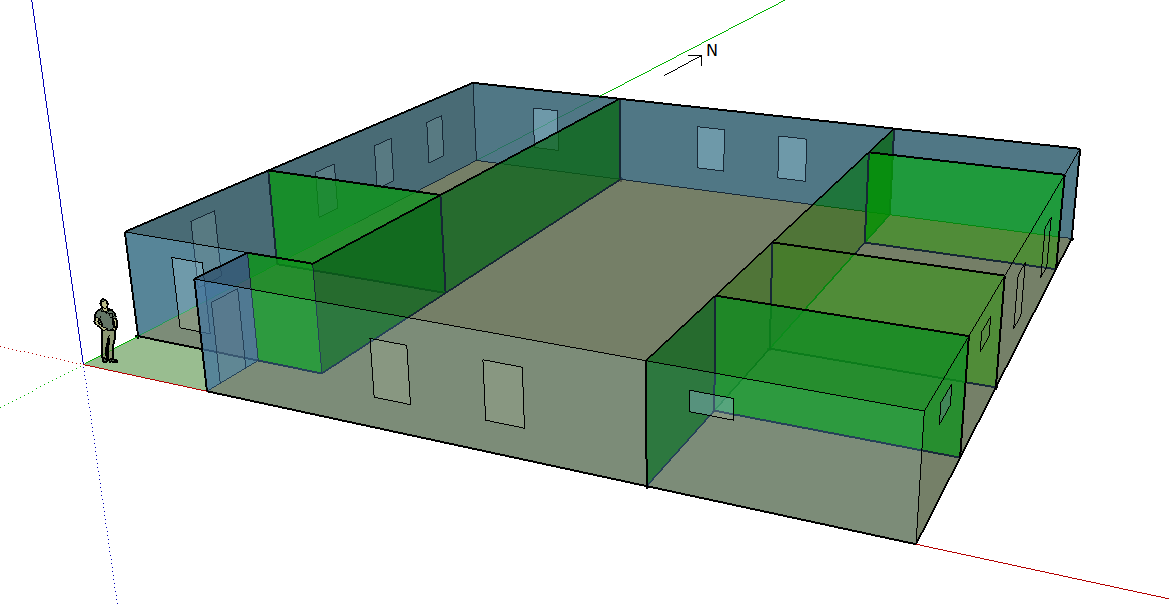
\includegraphics[scale=0.4]{vedlegg/DMozN.png}
    \caption{Building geometry}
    \label{fig:zones}
\end{figure}

\section{Building Envelope}
The U-values in the construction materials in the building envelope, simulated in EnergyPlus can be seen in table \ref{tab:Uvalue}.

\begin{table}[h!]
    \centering
        \caption{U-values, building envelope}
    \begin{tabular}{p{2cm}|p{1.8cm}|p{2cm}}
         \textbf{Surface} & \textbf{Thermal resistance} $\mathbf{[m^2}$\textbf{K/W]} & \textbf{U-value [W/} $\mathbf{m^2}$\textbf{K]} \\
         \hline
        Roof & 4.3564 & 0.2295  \\
        \hline
        External walls & 1.5106 & 0.6620 \\
         \hline
        Floor & 1.064 & 0.9397 \\
         \hline
         Windows & 0.4494 & 2.225 \\
    \end{tabular}
    \label{tab:Uvalue}
\end{table}

Comparing table \ref{tab:uvalue} and table \ref{tab:Uvalue}, the U values in the building envelope can be observed to be within Chinese governmental regulations.

\section{Thermal Zones}
The building is divided into different thermal zones according to the use of the room. The two restrooms are the only zones that are simulated based on the same criterias, but also there will two separate calculations be made.

\begin{figure}[h!]
    \centering
    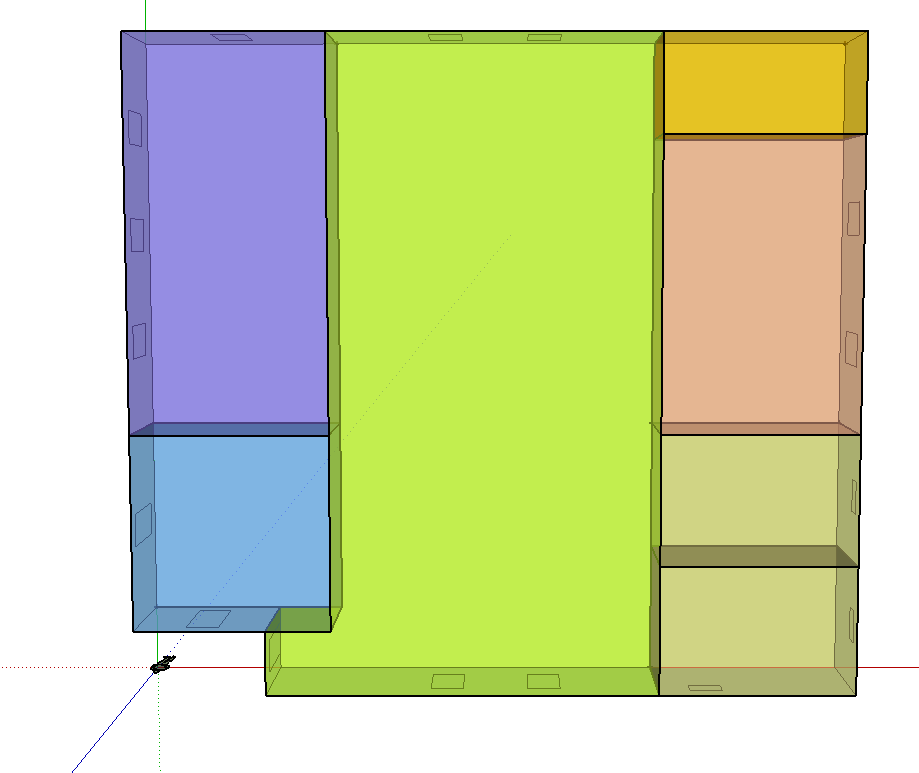
\includegraphics[scale=0.5]{vedlegg/zone.png}
    \caption{Caption}
    \label{fig:thermal}
\end{figure}

\section{HVAC}
It is assumed activity in the building between 08.00 and 16.00, with an activity level of 1.2 met. clothing level is assumed to be 1 clo all year around. Thermal comfort in the given conditions is between 22-24 degrees. 
\section{PV panels}
The roof has an area of 420m$^2$ where PV moduls will be placed

\section{Quality assurance}
\subsection{Verification}

To verify the model, certain parameters has been changed to analyze the impact on the simulation. Table \ref{tab:comp} shows the energy demand for heating and cooling at different heating and cooling setpoints. There is a lower total energy demand and peak load demand for both heating when heating setpoint temperature is 20$^o$C compared to 21$^o$C. The same accounts for total cooling demand and peak load for cooling when setpoint temperature for cooling is set to 26$^o$C, compared to 24.5$^o$C. These results is in accordance to what to expect in real life, and it is therefore a valid verification. 

\begin{table}[h!]
    \centering
        \caption{Energy demand for space heating and cooling at different setpoint temperatures}
    \begin{tabular}{|p{2.8cm}|p{1.8cm}|p{1.8cm}|}
         \hline
        & \textbf{Heating} & \textbf{Cooling} \\
        \hline
    \multicolumn{3}{|c|}{Heating setpoint 21$^O$C, cooling setpoint 24.5$^O$C} \\
    \hline
        \textbf{Total energy demand [kWh]} & 39013.6 & 24820.2 \\
        \hline
        \textbf{kWh/m$^2$} & 97.0  & 61.7 \\
        \hline
        \textbf{Peak load [kW]} & 19.9 & 37.1 \\
        \hline
    \multicolumn{3}{|c|}{Heating setpoint 20$^O$C, cooling setpoint 26$^O$C} \\
        \hline
        \textbf{Total energy demand [kWh]} & 26583.9 & 15959.7 \\
        \hline
        \textbf{kWh/m$^2$} & 63.3  & 38.0 \\
        \hline
        \textbf{Peak load [kW]} & 17.4 & 33.0 \\
        \hline
    \end{tabular}
    \label{tab:comp}
\end{table}

Table \ref{tab:com} shows simulations with different insulation thickness in the external wall. A thicker insulation thickness results in lower energy demand for heating and cooling, and a lower peak load demand. This is naturally exactly as expected and another good validation of the model. 

\begin{table}[h!]
    \centering
        \caption{Energy demand for space heating and cooling at different wall insulation thickness}
    \begin{tabular}{|p{2.8cm}|p{1.8cm}|p{1.8cm}|}
         \hline
        & \textbf{Heating} & \textbf{Cooling} \\
        \hline
    \multicolumn{3}{|c|}{External wall, insulation thickness 33.7mm} \\
        \hline
        \textbf{Total energy demand [kWh]} & 26583.9 & 15959.7 \\
        \hline
        \textbf{kWh/m$^2$} & 63.3  & 38.0 \\
        \hline
        \textbf{Peak load [kW]} & 17.4 & 33.0 \\
        \hline
    \multicolumn{3}{|c|}{External wall, insulation thickness 56.6mm} \\
        \hline
        \textbf{Total energy demand [kWh]} & 25810.4 & 15321.0 \\
        \hline
        \textbf{kWh/m$^2$} & 61.5  & 36.5 \\
        \hline
        \textbf{Peak load [kW]} & 16.9 & 32.3 \\
        \hline
    \end{tabular}
    \label{tab:com}
\end{table}

\subsection{Validation}

To validate the model, an analysis of the simulation was made to see if all design criteria was met. Table \ref{tab:valid} shows a summary of time the setpoint temperature was not met. The table indicates the temperatures was always within wanted parameters, which is a good validation that the model works exactly as it is intended to.

\begin{table}[h!]
    \centering
        \caption{Validation of operative temperature in the building}
    \begin{tabular}{|c|c|}
         \hline
        Time setpoint not met & hr  \\
         \hline
         During heating & 0.0 \\
         \hline
         During cooling & 0.0 \\
         \hline
    \end{tabular}
    \label{tab:valid}
\end{table}


\subsection{Calibration}


\chapter{Results} %\label{Resultat}
The results of the simulations done in EnergyPlus and TRNSYS will be presented in this chapter.

\section{Energy demand}
To calculate the energy demand for space heating and cooling, an ideal air load is used and the simulation result from EnergyPlus is shown in figure \ref{fig:hd}. This figure shows the total heating and cooling load for each month and the average outdoor air dry bulb temperature. 

\begin{figure}[h!]
    \centering
    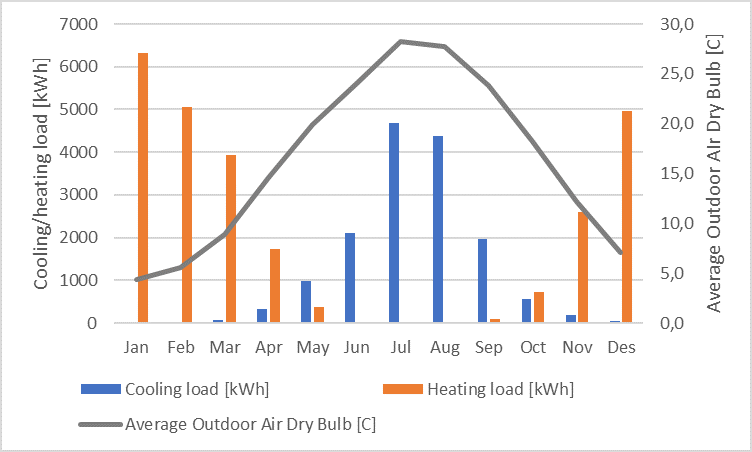
\includegraphics[scale=0.8]{vedlegg/combigraph.png}
    \caption{Heating load and cooling load vs average outdoor air dry bulb temperature, simulated in ENergyPlus}
    \label{fig:hd}
\end{figure}

Figure \ref{fig:ldch} displays hourly energy consumption for heating and cooling over a year. 

\begin{figure}[h!]
    \centering
    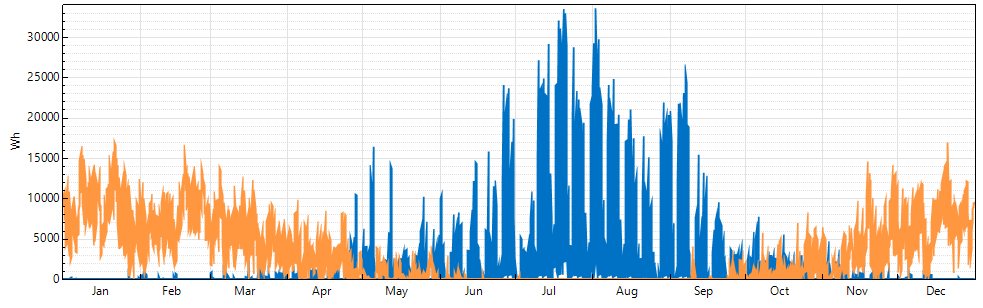
\includegraphics[scale=0.5]{vedlegg/coolheat.png}
    \caption{Energy consumption for heating and cooling, 1 hour time step.}
    \label{fig:ldch}
\end{figure}

Table \ref{tab:sum} gives a summary of the total energy demand for heating and cooling, the energy consumption per square meter and the peak load demand. 

\begin{table}[]
    \centering
        \caption{Summary of energy demand for space heating and cooling}
    \begin{tabular}{|p{2.5cm}|p{1.8cm}|p{1.8cm}|}
         \hline
        & \textbf{Heating} & \textbf{Cooling} \\
        \hline
        \textbf{Total energy demand [kWh]} & 25810.4 & 15321.0 \\
        \hline
        \textbf{kWh/m$^2$} & 61.5  & 36.5 \\
        \hline
        \textbf{Peak load [kW]} & 16.9 & 32.3 \\
        \hline
    \end{tabular}
    \label{tab:sum}
\end{table}

The hourly energy consumption from figure \ref{fig:ldch} gives a load duration curve for heating, figure \ref{fig:hload} and a load duration curve for cooling, figure \ref{fig:cload}.

\begin{figure}[h!]
    \centering
    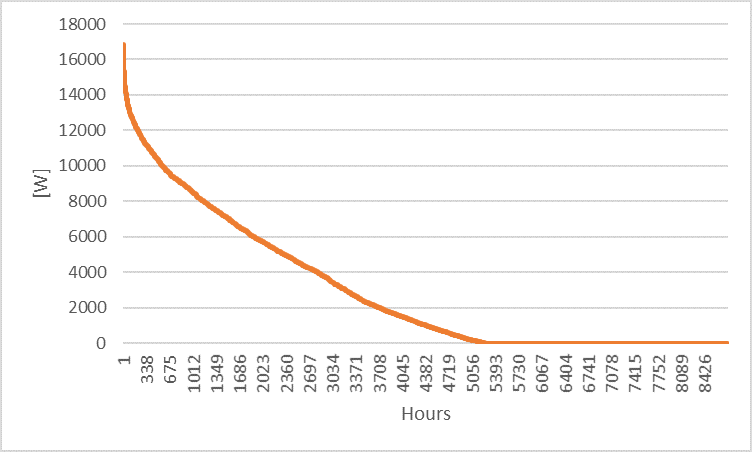
\includegraphics[scale=0.8]{vedlegg/hl1512.png}
    \caption{Load duration curve for space heating}
    \label{fig:hload}
\end{figure}

\begin{figure}[h!]
    \centering
    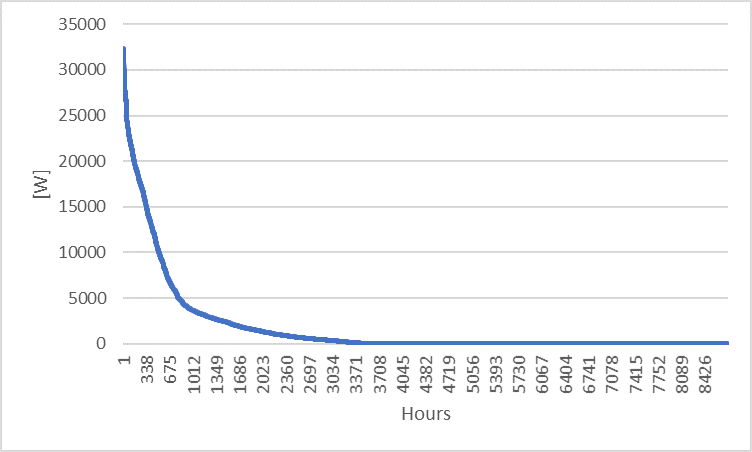
\includegraphics[scale=0.8]{vedlegg/cl1512.png}
    \caption{Load duration curve for space cooling}
    \label{fig:cload}
\end{figure}

\begin{table}[h!]
    \centering
       \caption{Caption}
    \begin{tabular}{|p{2cm}|p{2cm}|p{2cm}|p{2cm}|p{2cm}|p{2cm}|}
    \hline
        HP Capacity [kW] & Energy coverage Heating [\%]  & Energy coverage Cooling [\%] & Total energy coverage [\%] & Peak Load Coverage Heating [\%] & Peak Load Coverage Cooling [\%] \\
         \hline
          10 & 90.1 & 68.4 & 81.6 & 50.3& 27.0  \\
         \hline
         11 & 93.4 & 71.4 & 84.8 & 55.3 & 29.6   \\
         \hline
          12 & 95.8 & 74.3  & 87.4 &  60.3 & 32.3  \\
         \hline
          13 & 97.6 & 77.0 & 89.6 & 65.4 & 35.0 \\
         \hline
         14 & 98.8 & 79.5 & 91.3 & 70.3 & 37.7 \\
         \hline
         15 & 99.5 & 81.8 & 92.6 & 75.4 & 40.4  \\
         \hline
    \end{tabular}
    \label{tab:my_label}
\end{table}

An analysis of optimal angel for the PV panels was made and the result is displayed in figure \ref{fig:angel}. The result was an optimal angel of 22.5 degrees. 

\begin{figure}[h!]
    \centering
    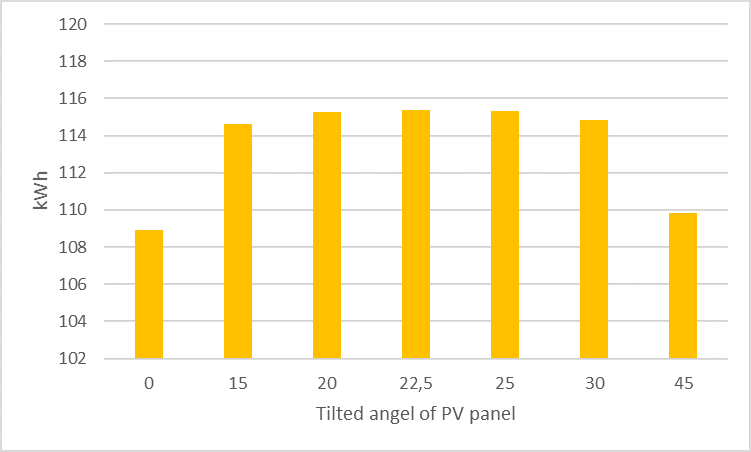
\includegraphics[scale=0.8]{vedlegg/angel.png}
    \caption{Analysis of optimal angel of PV panels, area = 0.89m$^2$, $\eta$ = 8.7\%}
    \label{fig:angel}
\end{figure}

\pagebreak



\chapter{Discussion}

\section{Heat Pump}

\begin{table}[h!]
    \centering
        \caption{Caption}
    \begin{tabular}{|p{2cm}|c|c|c|c|c|}
         \hline
         & \multicolumn{2}{c}{Model} & & MG-05KFXLR & MG-05KFXLR/380V \\
         \hline
        \multirow{6}{*}{Specifications} & \multirow{3}{*}{Heating mode} & Input power & [kW] & 3.49  & 4.09 \\
         \cline{3-6}
        & &Heating capacity& [kW] & 14 & 16.4 \\
        \cline{3-6} 
        & &COP & &4.01 & 4.01 \\
        \cline{2-6}
        & \multirow{3}{*}{Cooling mode} &Input power &[kW]  & 4.01 & 4.71\\
         \cline{3-6}
        & &Cooling capacity &[kW] & 11 & 12.8\\
        \cline{3-6}
        & &EER & & 2.74 & 2.72 \\
        \hline
        & & Price & [USD] & 9 800 & 10 800 \\
        \hline
    \end{tabular}
    \label{tab:hpchina}
    \end{table}
    
Assumtions made: COP = SCOP, Efficiency of boiler = 0.9
    
\begin{table}[h!]
    \centering
        \caption{Caption}
    \begin{tabular}{|c|c|c|c|c|}
         \hline
         \multicolumn{3}{|c|}{Model} & MG-05KFXLR & MG-05KFXLR/380V \\
         \hline
       \multirow{4}{*}{Heating mode} & Energy coverage & [\%] & 98.8  & \\
         \cline{2-5}
         & Energy demand HP & [kWh] & 9 592.9  &  \\
         \cline{2-5}
         & Energy demand peak load & [kWh] & 520.2  & \\
        \cline{2-5}
         & Total energy demand & [kWh] & 10 113.1 &  \\
        \cline{1-5}
         \multirow{4}{*}{Cooling mode} & Energy coverage &[\%]  & 71.4 & \\
         \cline{2-5}
         & Energy demand HP & [kWh] & 6467.7 & \\
        \cline{2-5}
        & Energy demand peak load & [kWh] & 7887.2 & \\
        \cline{2-5}
         & Total energy demand & [kWh] & 14 354.9  &  \\
         \hline
         & Total energy demand & [kWh] & 24 468  &  \\
         \hline
         & Energy saved  & [\%] &  62\% &   \\
         \hline
    \end{tabular}
    \label{tab:hpchina}
\end{table}



\chapter{Conclusion}

\chapter{Further work}

\newpage

\printacronyms[include-classes=abbrev,name=Abbreviations]

\printacronyms[include-classes=nomencl,name=Nomenclature]

\newpage

\chapter*{Appendix}
\begin{table}[h!]
    \centering
        \caption{Thermal resistance, floor}
    \begin{tabular}{p{2cm}|p{1.8cm}|p{2.5cm}|p{2cm}}
         \textbf{Material} & \textbf{Thickness [m]} & \textbf{Conductivity} [W/mK] & \textbf{Thermal resistance [$m^2$K/W]} \\
         \hline
         8in Concrete HW & 0.2033 & 1.7296 & 0.11754 \\
         \hline
         I01 25mm insulation board & 0.0254 & 0.03 & 0.84667 \\
         \hline
         CP02 Carpet Pad & - & - & 0.1 \\
         \hline
         \textbf{Total} & 0.2287 & & 1.064 \\
    \end{tabular}
    \label{tab:Rvalue, floor}
\end{table}

\begin{table}[h!]
    \centering
        \caption{Thermal resistance, external wall}
    \begin{tabular}{p{2cm}|p{1.8cm}|p{2.5cm}|p{2cm}}
         \textbf{Material} & \textbf{Thickness [m]} & \textbf{Conductivity} [W/mK] & \textbf{Thermal resistance [$m^2$K/W]} \\
         \hline
         1in Stucco & 0.0253 & 0.6916 & 0.036571 \\
         \hline
         8in Concrete HW & 0.2033 & 1.7296 & 0.11754 \\
         \hline
         Wall Insulation & 0.0566 & 0.04432 & 1.27708 \\
         \hline
         1/2in Gypsum & 0.0127 & 0.16 & 0.079375 \\
         \hline
         \textbf{Total} & 0.2979 & & 1.51056 \\
    \end{tabular}
    \label{tab:Rvalue, wall}
\end{table}

\begin{table}[h!]
    \centering
        \caption{Thermal resistance, roof}
    \begin{tabular}{p{2cm}|p{1.8cm}|p{2.5cm}|p{2cm}}
         \textbf{Material} & \textbf{Thickness [m]} & \textbf{Conductivity} [W/mK] & \textbf{Thermal resistance [$m^2$K/W]} \\
         \hline
         Roof Membrane & 0.095 & 0.16 & 0.059375 \\
         \hline
         Roof Insulation & 0.2105 & 0.049 & 4.29592 \\
         \hline
         Metal Decking & 0.0015 & 1.311 & 0.00114 \\
         \hline
         \textbf{Total} & 0.2215 & & 4.35644 \\
    \end{tabular}
    \label{tab:Rvalue, roof}
\end{table}

\begin{table}[h!]
    \centering
        \caption{Thermal resistance, windows}
    \begin{tabular}{p{2cm}|p{1.8cm}|p{2.5cm}|p{2cm}}
         \textbf{Material} & \textbf{Thickness [m]} & \textbf{Conductivity} [W/mK] & \textbf{Thermal resistance [$m^2$K/W]} \\
         \hline
         Glass & 0.004 & 0.0089 & 0.44944 \\
         \hline
         \textbf{Total} & 0.004 & 0.0089 & 0.44944 \\
    \end{tabular}
    \label{tab:Rvalue, windows}
\end{table}

%\begin{figure}[h!]
  %  \begin{center}
  %  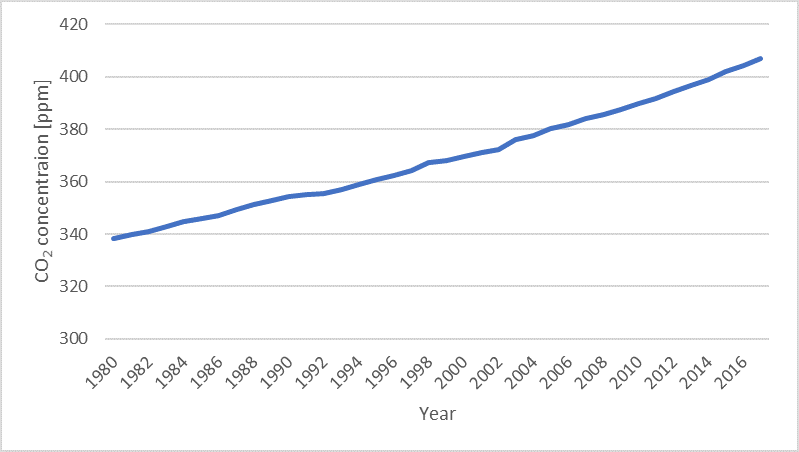
\includegraphics[scale=0.75]{vedlegg/co2new}
  % \caption{CO$_2$ Concentration in the atmosphere from 1980 - 2017}
  %  \label{fig:co2}
  %  \end{center}
%\end{figure}

%\begin{figure}[h!]
 %   \begin{center}
 %   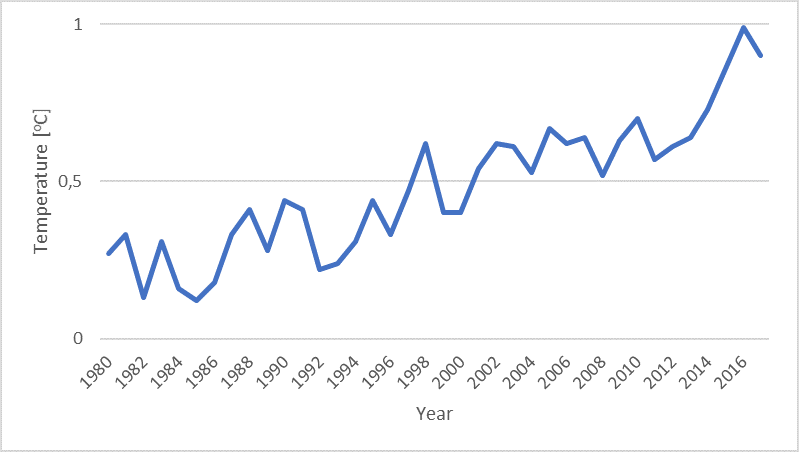
\includegraphics[scale=0.75]{vedlegg/tempnew}
 %   \caption{Temperature from 1980 - 2017 compared to pre-industrail levels}
 %   \label{fig:temp}
 %   \end{center}
%\end{figure}



\begin{thebibliography}{1}

\bibitem{Enok} Novakovic, V., Hanssen, S.O., Thue, J.V., Wangensteen I., Gjerstad, F.O., et al.(2007) \textit{Energy management in buildings}. 3. Edition. Gyldendal Norsk Forlag AS 

\bibitem{ETP} International Energy Agency (2017) \textit{Energy Technology Perspectives 2017
Catalysing Energy Technology Transformations} %https://www.iea.org/buildings/

\bibitem{co2levels} Dlugokencky, E (5 February 2016). \textit{Annual Mean Carbon Dioxide Data}. Earth System Research Laboratory. National Oceanic \& Atmospheric Administration. Retrieved 30 september 2018

\bibitem{paris} United Nations (2015). \textit{Paris Agreement}

\bibitem{stats} International Energy Agancy (2017). \textit{Key world
energy statistics}.

\bibitem{temp} NASA's Goddard Institute for Space Studies (2017) \textit{GLOBAL LAND-OCEAN TEMPERATURE INDEX}.  Retrieved 30 september 2018 %https://climate.nasa.gov/vital-signs/global-temperature/

\bibitem{Ipcc}  Intergovernmental  Panel  on  Climate  Change (2018) \textit{SR 1.5}

\bibitem{Nhaps} Nature Publishing Group (2001). \textit{The National Human Activity Pattern Survey (NHAPS): a resource for assesing exposure to environmental pollutants}

\bibitem{uvalue} Ministry of Housing and Urban-Rural Development of the People's Republic of China (2005). \textit{Design Standard for Energy Efficiency of Public Buildings - GB 50189-2005}
% http://www.gbpn.org/databases-tools/bc-detail-pages/china-public#Energy%20Covered

\bibitem{energyplus} The U.S. Department of Energy’s (DOE) Building Technologies Office (BTO), managed by the National Renewable Energy Laboratory (NREL) \textit{EnergyPlus}

\bibitem{dahl} Dahl T., Albjerg N, et. al., (2010) \textit{Climate and Architecture}. Routledge. 

\bibitem{temp} Holiday weather % https://www.holiday-weather.com/shanghai/averages/

\end{thebibliography}


\pagestyle{empty}
\includepdf[pages={2}, pagecommand={}]{vedlegg/Cover.pdf}
\clearpage
\thispagestyle{empty}

\end{document}